\documentclass{beamer}
\title{Snails}
\author{Craig \and Milan \and Jack}
\date{20th June}
\usetheme{AnnArbor}
\usecolortheme{dolphin}
\setbeamertemplate{navigation symbols}{} 

\AtBeginSection
{
  \begin{frame}{Outline}
    \tableofcontents[currentsection]
  \end{frame}
}

\defbeamertemplate*{footline}{my infolines theme}
{
    \leavevmode%
        \hbox{%
            \begin{beamercolorbox}[wd=.333333\paperwidth,ht=2.25ex,dp=1ex,center]{author in head/foot}%
                \usebeamerfont{author in head/foot}\insertshortauthor~~\insertshortinstitute
                \end{beamercolorbox}%
                \begin{beamercolorbox}[wd=.333333\paperwidth,ht=2.25ex,dp=1ex,center]{title in head/foot}%
                \usebeamerfont{title in head/foot}\insertshorttitle
                \end{beamercolorbox}%
                \begin{beamercolorbox}[wd=.333333\paperwidth,ht=2.25ex,dp=1ex,right]{date in head/foot}%
                \usebeamerfont{date in head/foot}\insertshortdate{}\hspace*{2em}
            \insertframenumber{} / \inserttotalframenumber\hspace*{2ex} 
            \end{beamercolorbox}}%
                \vskip0pt%
}

\begin{document}

\begin{frame}
  \titlepage
  \vspace{\baselineskip}
  \begin{center}
    
\includegraphics[scale=0.15]{snail_teeth.png}
  \end{center}
\end{frame}

\section{Introduction}

\begin{frame}{Introduction}
  TODO:\\
  \vspace{\baselineskip}
  We did a game about snails and we think it is pretty cool and you guys should probably check it out or something.\\
  \vspace{\baselineskip}
  I mean, no pressure, but it is pretty awesome.
\end{frame}


\section{The Game}
\subsection{Game Background}

\begin{frame}{Background Story}
  Players are ghosts, in a haunted house which is under attack from evil giant snails.\\
  Ghosts must wear their magic hats at all times to 'live'. The hats magically allow them to interact with the physical world (hold guns, ammo, etc), which also means that the ghosts cannot pass through walls. The hats also magically tie the ghosts to the house - they must haunt the same place forever.\\
  The snails are slightly magical, and are the only things that can kill the ghosts.\\
  \vspace{\baselineskip}
  \begin{figure}
    \hfill
    
\includegraphics[scale=0.15]{snail_teeth_flip.png}
  \end{figure}
\end{frame}

\begin{frame}{Game Rules}
  \begin{itemize}
    \item Ghosts may chose one action to do per turn:
      \begin{itemize}
        \item Move
        \item Shoot
        \item Reload
        \item Pick up or drop the ammo box
        \item Create or fix a barricade
        \item Destroy a barricade
      \end{itemize}
  \end{itemize}
\end{frame}

\begin{frame}{Game Rules}
  \begin{itemize}
    \item Players have limited ammo, and may not shoot when they have none left
    \item Players carrying the ammo box may only either move or drop the ammo box on their turn
    \item Players may not reload from a carried ammo box
    \item Players may not create or repair a barricade when there are snails in the adjacent room
    \item After each player has had their turn, snails will either chose to chase the nearest player, or move randomly
    \item Ghosts will die when in a room with any number of snails
  \end{itemize}
\end{frame}

\subsection{Aesthetics}

\begin{frame}{Art and Animation}
  \begin{center}
    
\includegraphics[scale=0.15]{snail_teeth.png}
    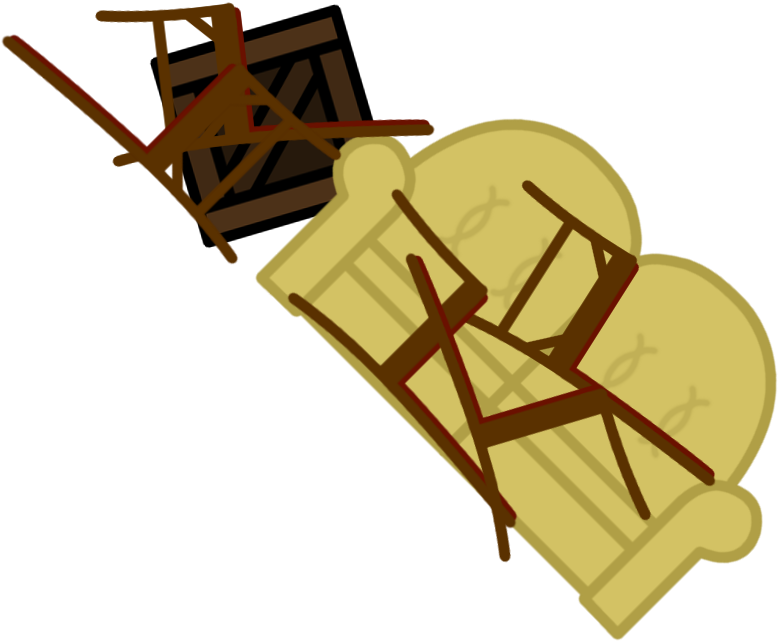
\includegraphics[scale=0.1]{../game/static/img/barricade_stairs.png}
    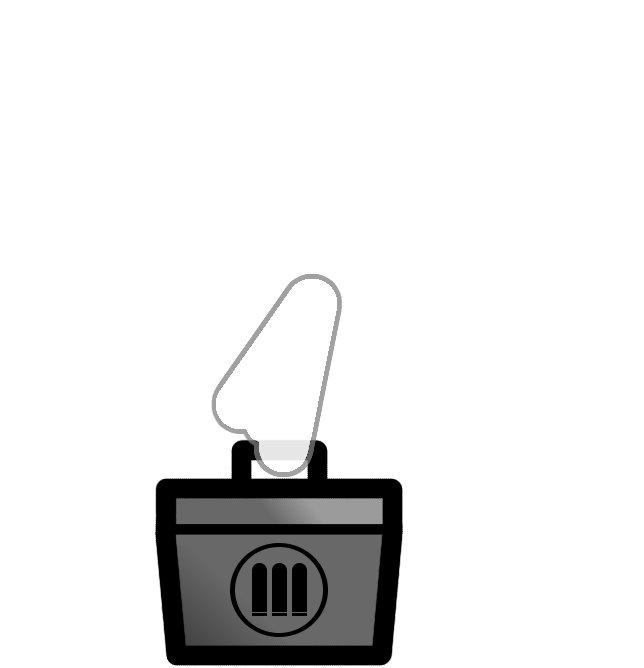
\includegraphics[scale=0.1]{../game/static/img/ghost_ammobox.png}
    
\includegraphics[scale=0.15]{snail_teeth.png} \\
    Various graphics created for the game
  \end{center}
  \begin{itemize}
    \item Art - GIMP
      \hfill
      
\includegraphics[scale=0.025]{gimp_logo.png}
    \item Animation - JavaScript/paper.js
      \hfill
      
\includegraphics[scale=0.4]{paper_logo.png}
      \begin{itemize}
        \item (see Client Implementation for optimisations)
      \end{itemize}
  \end{itemize}
\end{frame}

\begin{frame}{User Interface}
  \begin{center}
    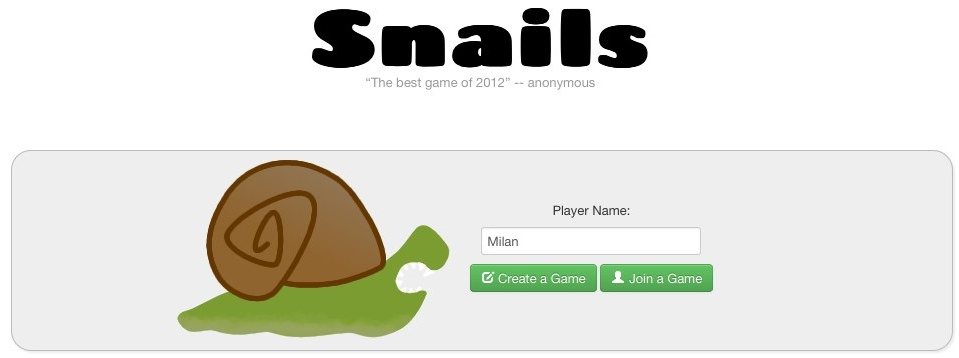
\includegraphics[scale=0.35]{index.jpg} \\
    Main screen
  \end{center}
\end{frame}

\begin{frame}{User Interface}
  \begin{center}
    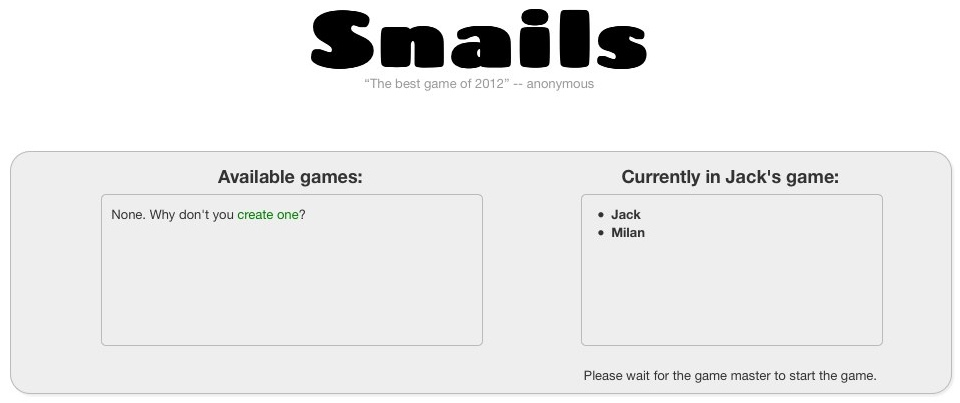
\includegraphics[scale=0.35]{join.jpg} \\
    Joining a game
  \end{center}
\end{frame}

\begin{frame}{User Interface}
  \begin{center}
    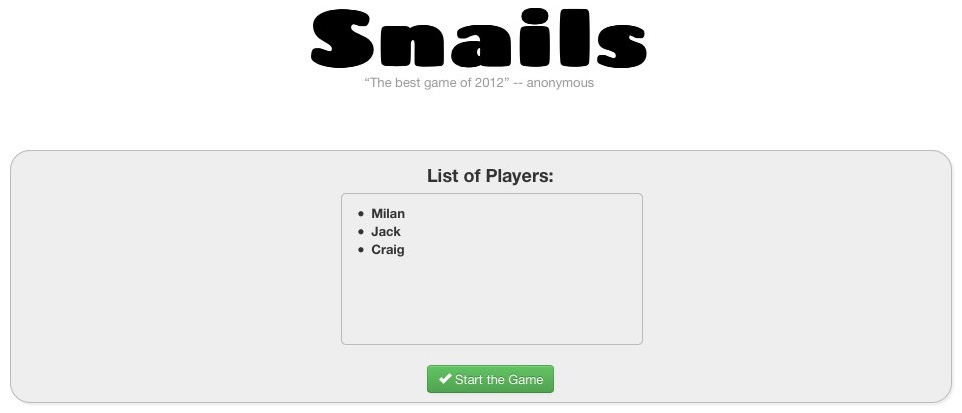
\includegraphics[scale=0.35]{create.jpg} \\
    Creating a new game
  \end{center}
\end{frame}


\section{Group Management}

\begin{frame}{Group Responsibilities}
  \begin{itemize}
    \item Milan: Website layout, server side code.
    \item Jack: Client side game representation, game ideas/rules development, animation
    \item Craig: Artwork, animation, game ideas/rules development
  \end{itemize}
\end{frame}

\begin{frame}{Pivotal Tracker}
  Tool for project management and collaboration. \\ 
  \begin{center}
    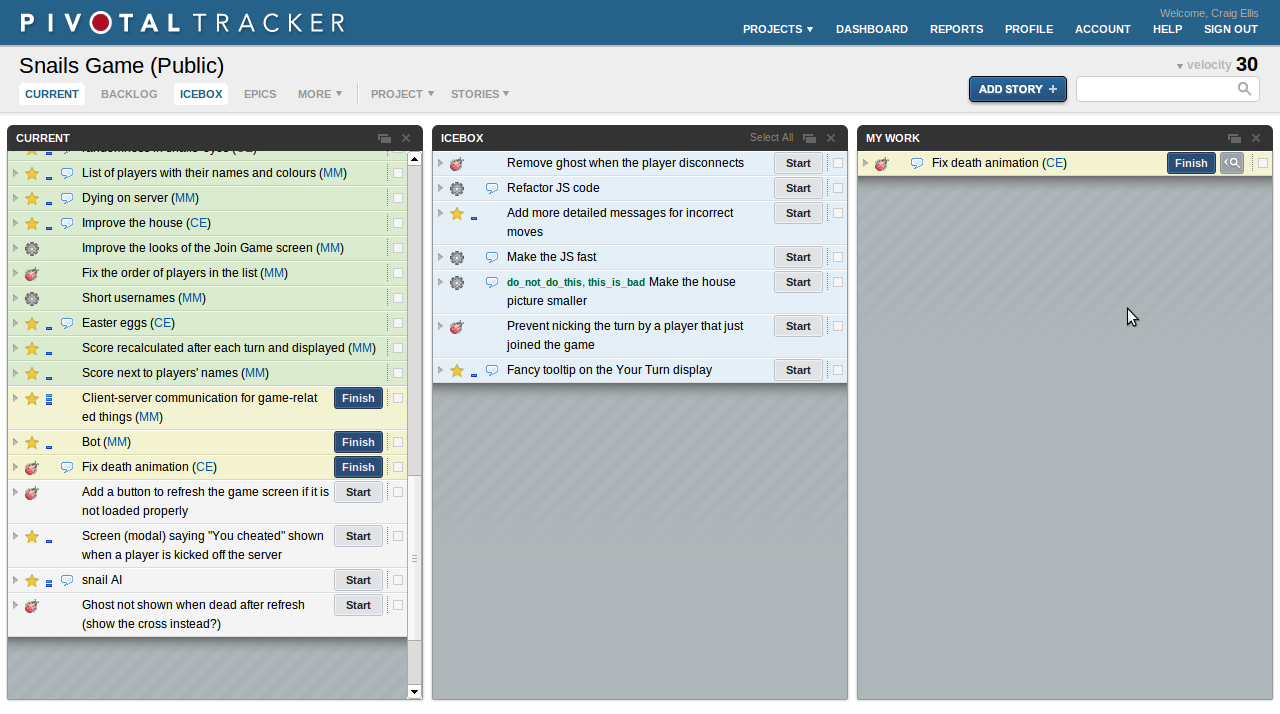
\includegraphics[scale=0.25]{pivotal.png} \\
    Pivotal Tracker main screen
  \end{center}
\end{frame}

\begin{frame}{Pivotal Tracker}
  \begin{center}
    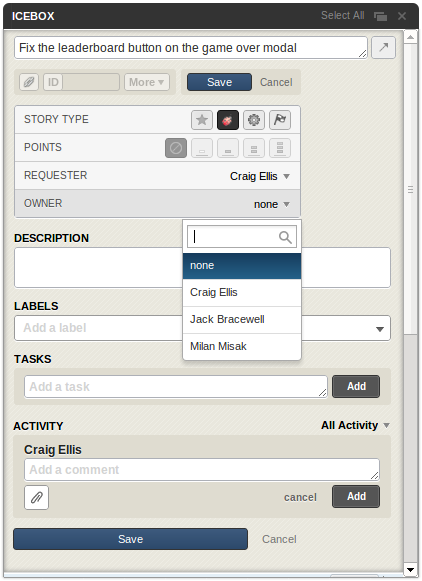
\includegraphics[scale=0.32]{pivotal_new_story.png} \\
    Creating a new story
  \end{center}
\end{frame}


\section{Implementation}
\subsection{Client}

\begin{frame}{Javascript}
  TODO:
  [insert map of components and interactions.]
  \begin{itemize}
    \item Only client side script supported by all browsers
    \vspace{\baselineskip}
    \item More stable than using plugins
    \vspace{\baselineskip}
    \item HTML5 graphics libraries available (we used paper.js)
  \end{itemize}
\end{frame}

\begin{frame}{JavaScript/HTML5 interaction}
  \begin{center}
    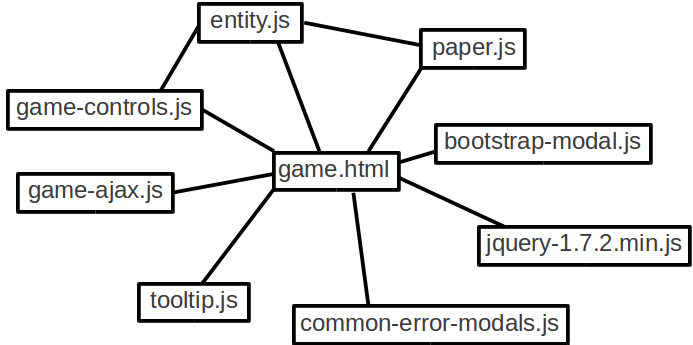
\includegraphics[scale=0.4]{game_html_structure.png} \\
    game.html structure
  \end{center}
\end{frame}

\begin{frame}{HTML5}
  \begin{itemize}
    \item Technology for the future
    \vspace{\baselineskip}
    \item No need to install plugins with modern broswers
    \vspace{\baselineskip}
    \item Faster, less likely to crash than plugins
  \end{itemize}
  \vspace{\baselineskip}
  \begin{center}
    
\includegraphics[scale=0.1]{HTML5_Logo_512.png}
  \end{center}
\end{frame}

\begin{frame}{Other useful things}
  jQuery, Twitter Bootstrap, 960.gs
\end{frame}

\begin{frame}{Graphics Optimisation}
  \begin{figure}[Snails]
    \centering
    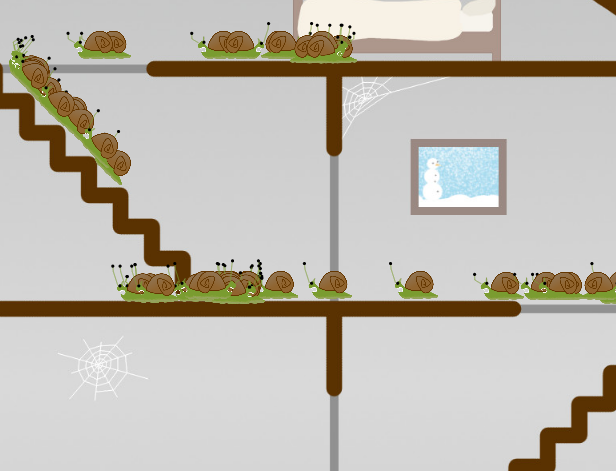
\includegraphics[scale=0.25]{SnailsScreenshot.png}
  \end{figure}
  \begin{itemize}
    \item Render eye movement every 3 frames.
    \item Cache snails as symbols.
    \item Movement calm down
  \end{itemize}
\end{frame}

\subsection{Server}

\begin{frame}{Backend Overview}
  [insert map of components and interactions.]
\end{frame}

\begin{frame}{Django}
  Web framework for Python \\
  \vspace{\baselineskip}
  \begin{itemize}
    \item Powerful ORM (object relational mapping)
    \vspace{\baselineskip}
    \item Template system
    \vspace{\baselineskip}
    \item Rapid development
  \end{itemize}
  \vspace{\baselineskip}
  \begin{center}
    
\includegraphics[scale=0.05]{django.png} \\
  \end{center}
\end{frame}

\begin{frame}{Heroku}
  Webhosting solution \\
  \vspace{\baselineskip}
  \begin{itemize}
    \item Supports Python/Django + many other frameworks, unlike DoC\ldots
    \vspace{\baselineskip}
    \item Easy deployment -- just push to a git repository
    \vspace{\baselineskip}
    \item Free plan available
  \end{itemize}
  \vspace{\baselineskip}
  \begin{center}
    
\includegraphics[scale=0.25]{heroku.png} \\
  \end{center}
\end{frame}

\begin{frame}{Xeround}
  Database-as-a-service -- MySQL \\
  \vspace{\baselineskip}
  Some say that an external DB is faster than Heroku's own PostgreSQL
  \vspace{\baselineskip}
  \begin{center}
    
\includegraphics[scale=0.25]{xeround.png} \\
  \end{center}
\end{frame}

\begin{frame}{Snail AI}
  \begin{itemize}
    \item Searching for ghosts: breadth-first search limited to depth of 5
    \vspace{\baselineskip}
    \item Random moves from time to time
    \vspace{\baselineskip}
    \item Caching of best actions for use by other snails in the same room
  \end{itemize}
\end{frame}

\section{Possible Extensions}
\begin{frame}{Possible Extensions}
  \begin{itemize}
    \item Chat Feature.
    \vspace{\baselineskip}
    \item Sound Effects.
    \vspace{\baselineskip}
    \item Animations for barricade destruction.
    \vspace{\baselineskip}
    \item Implement snails scaling the walls of the house and entering through the windows.
  \end{itemize}
\end{frame}

\section{Conclusion}

\begin{frame}{Conclusion}
  We are glad to have chosen languages we didn't know; it has been a worthwhile learning experience.\\
  \vspace{\baselineskip}
  Discovering Pivotal Tracker earlier could have improved team co-ordination from the start.\\
  \vspace{\baselineskip}
  In retrospect, it might have been better to save time by not creating all the artwork ourselves.
\end{frame}

\end{document}
